\documentclass[11pt]{beamer}

\usetheme{Antibes}
\usecolortheme{spruce}


\usepackage{amsfonts}
\usepackage{graphicx}
\usepackage{amsmath}
\usepackage{amssymb}
\usepackage{mathrsfs}
\usepackage{slashed}
\usepackage{xcolor}
\usepackage{multicol}

\setbeamertemplate{frame numbering}{fraction}


\title{Effective field theory approach to the Dark Matter indirect detection.}

\author{Md. Ehsanuzzaman}

\institute{Department of Physics\\University of Dhaka\\ Registration no: 2013-812-571 (2013-14)}

\date{}

\begin{document}

\begin{frame}
\titlepage
\end{frame}

 
%\begin{frame}
%\tableofcontents
%\end{frame}

%\begin{frame}{Evidence for Dark Matter}
%
%
%
%\textbf{Rotation curves:}  The constant nature of the orbital speed of the outer objects in this clusters indicates the incongruity in the mass concentration. Study the rotation curves of the galaxy clusters suggests that the mass concentration $\rho(r) \propto \frac{1}{r^2} $.
%
%
%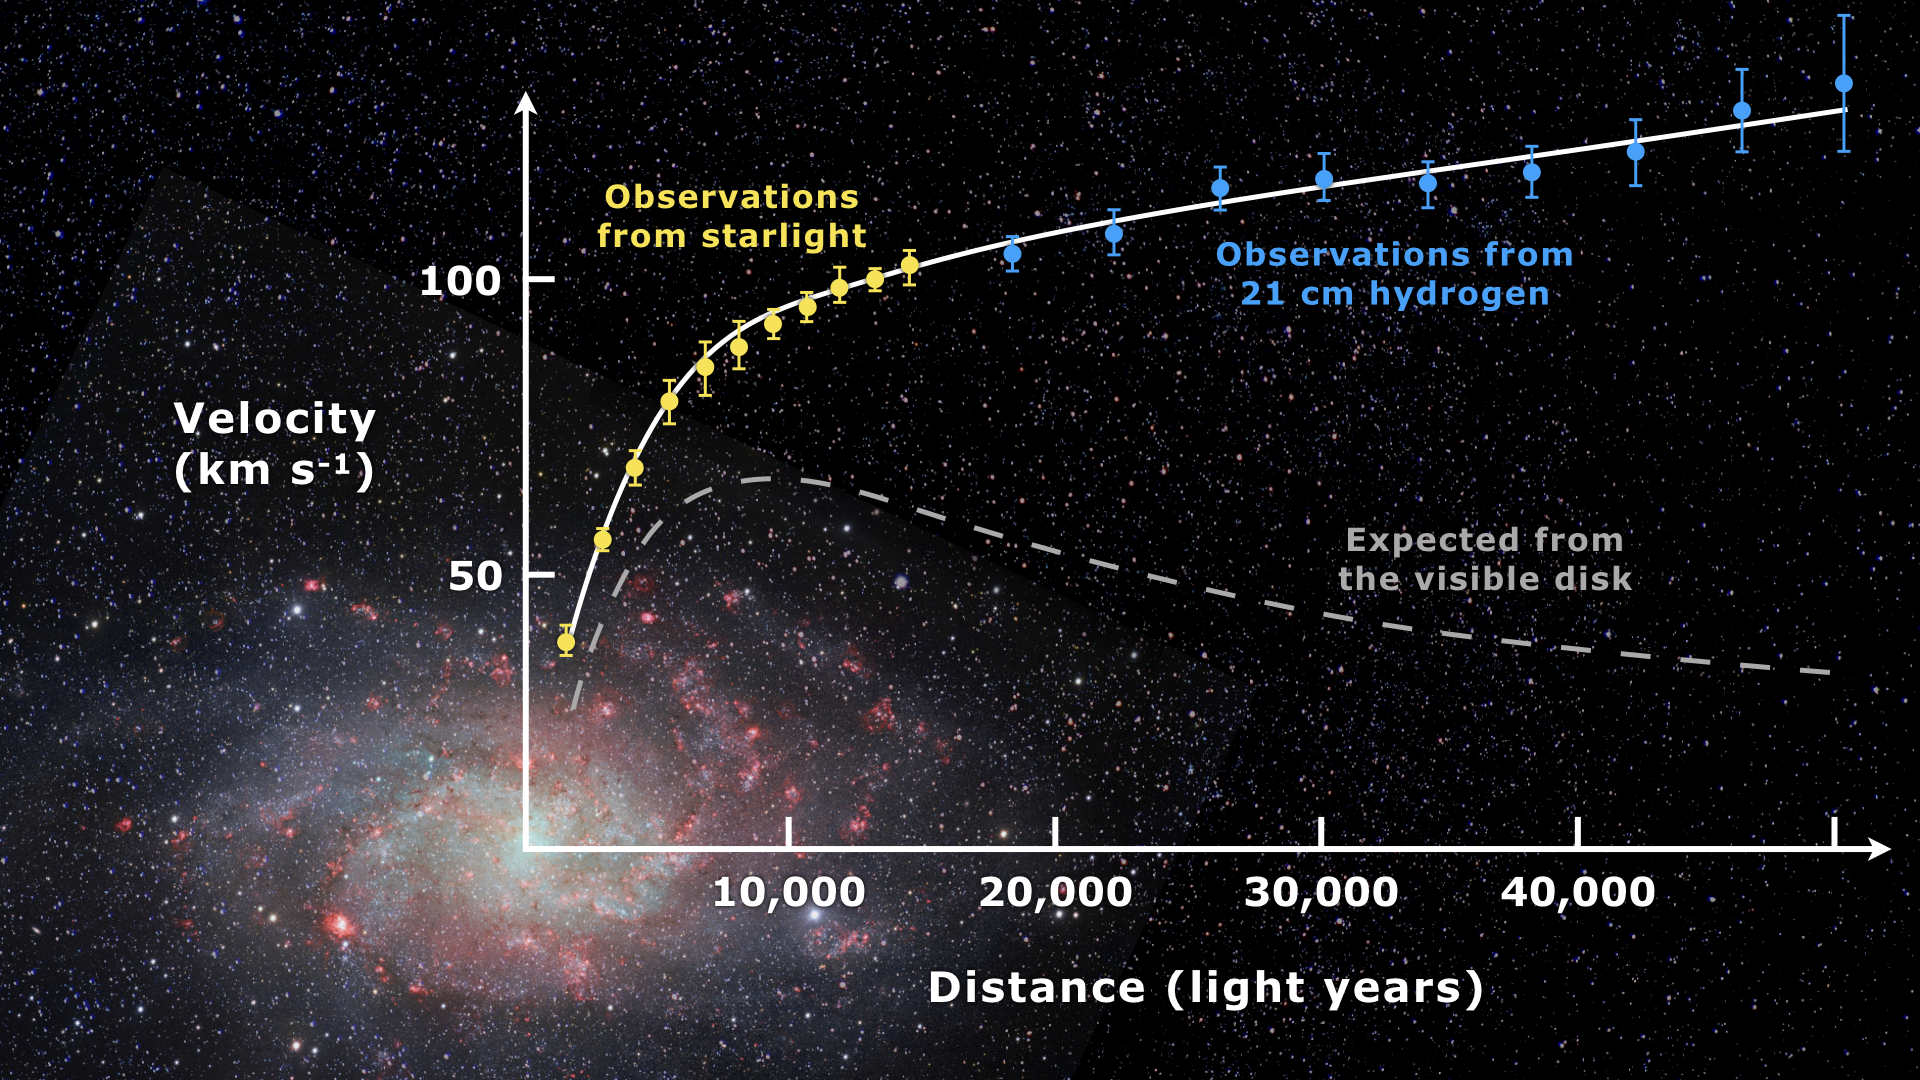
\includegraphics[scale=0.1]{R.png}
%
%
%\end{frame}
\begin{frame}{Contents}
\tableofcontents



\setcounter{page}{1}
\end{frame}




\begin{frame}{Evidence for Dark Matter : Rotation curves}
\section{Evidence for Dark Matter}

\subsection{Rotation curves}
\begin{small}
\begin{columns}

\begin{column}{0.6\textwidth}



\begin{itemize}
\item If we consider the radial velocity, $v$ of outermost star in a galaxy we get from the relation $\frac{mv^2}{r}= \frac{GMm}{r^2}$,
$$\Rightarrow  v\propto \frac{1}{\sqrt{r}}.$$
\vspace{-0.5cm}
%\item The orbital speed of the outer most stars with speed $v$ and radial distance $r$ of a galaxy cluster should have the following relations
 %$ v\propto \frac{1}{\sqrt{r}}$.
  
\item But from observations, we get $v(r)= constant$ of the outer most stars in the galaxy clusters. \textcolor{blue}{\tiny{ApJ., {\bf 39}, 137 (2001) }}
\item \textcolor{red}{So we can deduce that at the outermost region $M(r) \propto r$ which indicates an extended dark matter halo outside the visible disk of the galaxy.}
\end{itemize}

\end{column}

\begin{column}{0.5\textwidth}
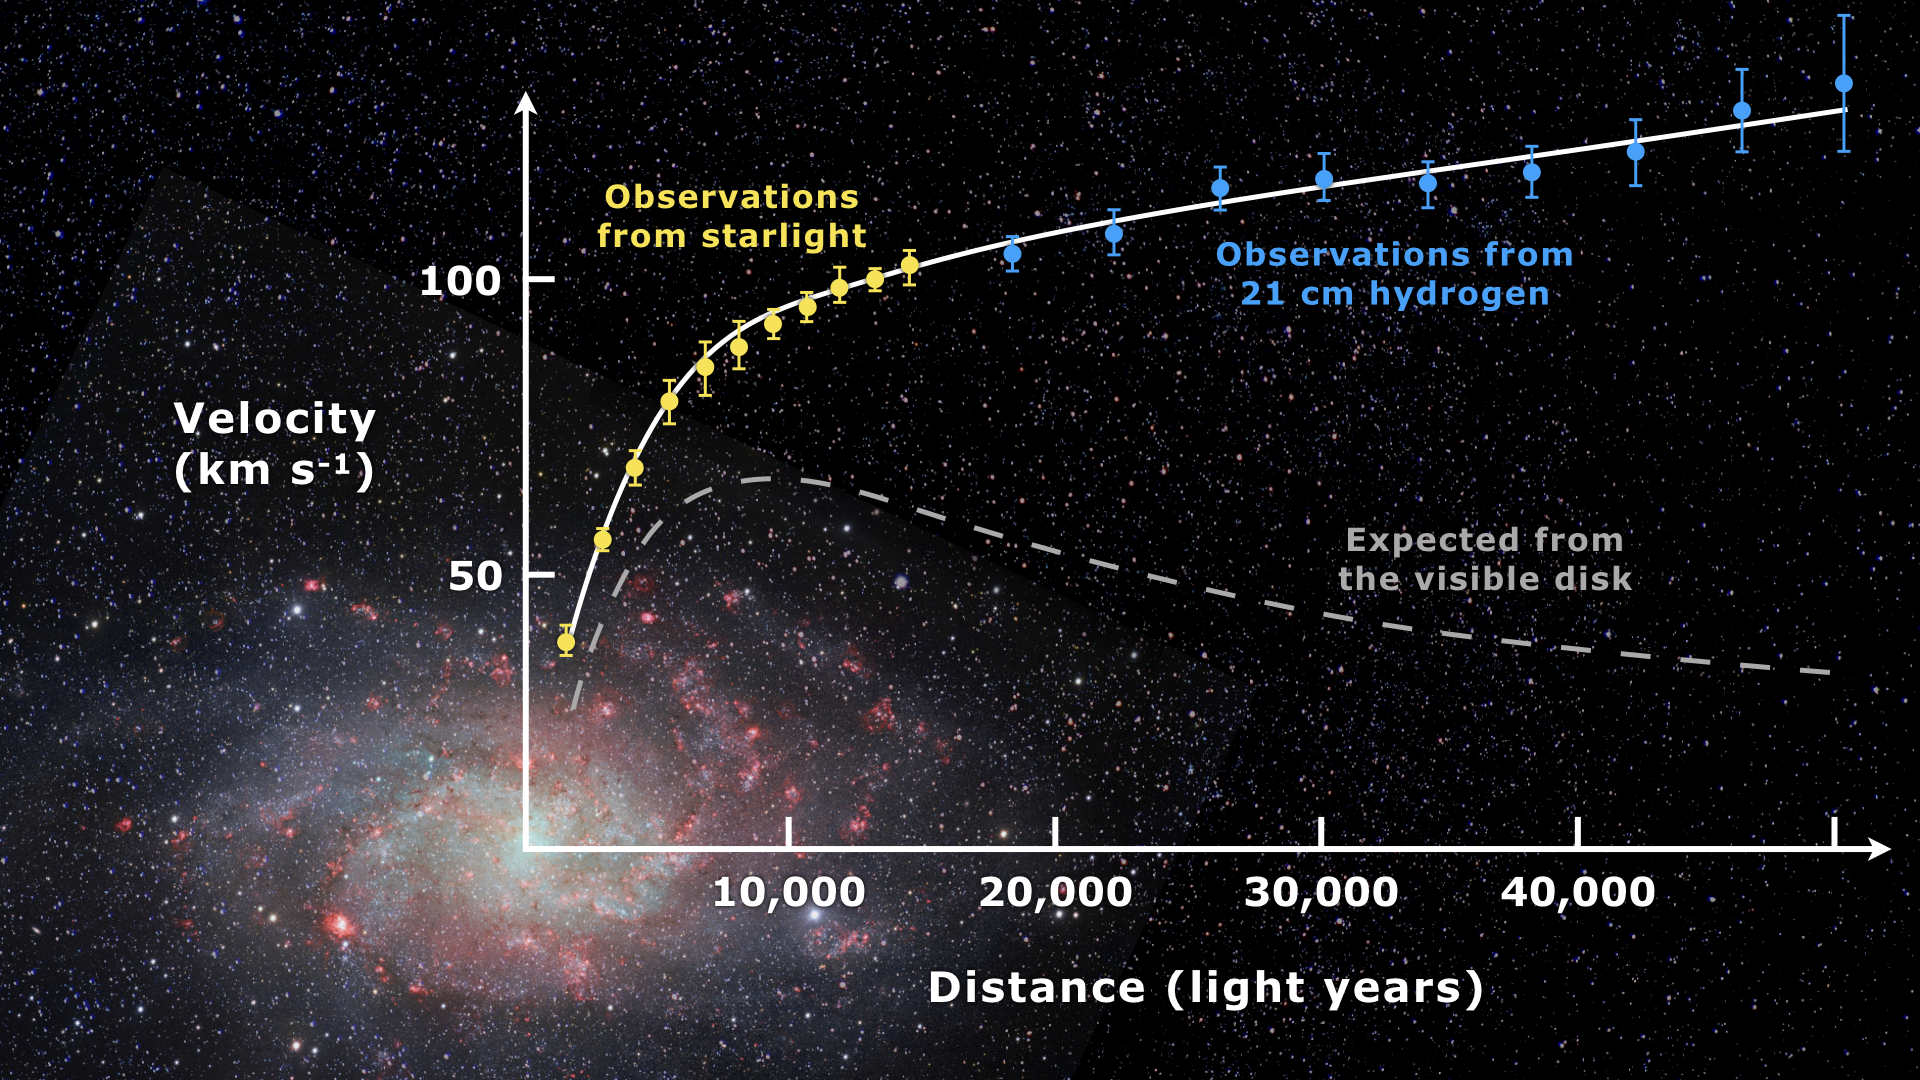
\includegraphics[scale=0.08]{R.png}
\end{column}


\end{columns}
\end{small}
\end{frame}



%\begin{frame}
%
%\begin{small}
%\textbf{Acoustic oscillation:} When the universe was 300,000 years old, matter and photon were tightly glued together. At that epoch the gravitational attraction created by Dark matter resulted in gravitational infall and created a sound wave. There were fluctuations in this gravitational field and these fluctuations are also imprinted on the energy spectrum of the Cosmic Microwave Background. From this CMB multipole moment energy spectrum we can compute the relic abundance of Dark matter which we now know from Planck Collaboration $\Omega_{DM} h^2 \sim 0.120 ± 0.001$.
%\end{small}
%
%\begin{center}
%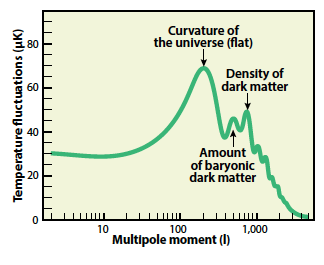
\includegraphics[scale=0.5]{cmb.png}
%\end{center}
%
%\end{frame}

\begin{frame}{Evidence for Dark Matter : Acoustic oscillation}
\subsection{Acoustic oscillation}

\begin{columns}
\begin{column}{0.6\textwidth}
\begin{itemize}
\item When the universe was around 300,000 years old, the information regarding the abundane of various matter content was imprinted on the CMB temperature as fluctuations.
\item \textcolor{red}{ From this CMB multipole moment temperature spectrum we can compute the relic abundance of Dark matter which we now know from Planck Collaboration $\Omega_{DM} h^2 \sim 0.120 \pm 0.001$.}
\end{itemize}

\end{column}


\begin{column}{0.5\textwidth}
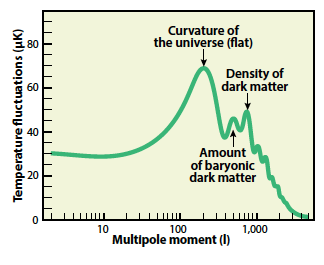
\includegraphics[scale=0.5]{cmb.png}
\end{column}

\end{columns}

\end{frame}







%\begin{frame}{Evidence for Dark Matter}
%
%\begin{tiny}
%\begin{itemize}
%\item \textbf{Gravitational lensing:} The most prolific evidence of DM was discovered using gravitational lensing phenomena in ”Bullet cluster”. Two galaxy clusters collided with each other about 4 billion
%light years away from earth at the constellation Carina and created the Bullet
%cluster. What happened is that
%the smaller cluster passed through the bigger one. From X-ray analyses, baryonic
%mass distribution was deduced and weak and strong lensing phenomena gave the
%DM distribution. While passing through, the smaller cluster was colliding with
%the bigger one, the shape of the smaller cluster became bullet like due to the
%enormity of the collision. Evidence suggests that the collision was so enormous
%that the baryonic matter was distorted and displaced from its dark matter halo.
%But the dark matter halo just passed through each other. 
%\end{itemize}
%\end{tiny}
%
%
%\begin{center}
%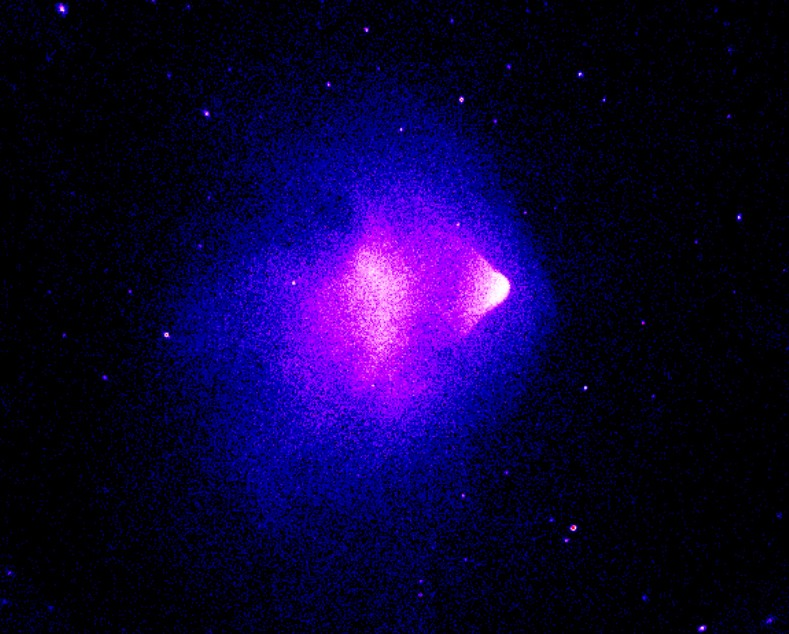
\includegraphics[scale=0.2]{bclstr.jpg}
%\end{center}
%\end{frame}


\begin{frame}{Evidence for Dark Matter : Gravitational lensing}

\subsection{Gravitational lensing}

\vspace{-0.3cm}

\begin{columns}
\begin{column}{0.6\textwidth}
\begin{small}
\begin{itemize}
\item The Bullet cluster ($1E0657-56$) was formed from  the collision between two galaxy clusters.  \textcolor{blue}{\tiny{ApJ.,{\bf 496}, L5 (1998)}}
\item From X-ray observation it was seen that the baryonic matter distribution has a distorted shape because of strong electromagnetic collisions among themselves. 
%\item While passing through, the shape of the smaller cluster became bullet-like due to the enormity of the collision among baryonic matter.
\item  \textcolor{green}{From Gravitational lensing observations the Dark Matter distribution was inferred.}

\item The spatial offset of the center of total mass from the center of baryonic center of mass peaks can be explained the existence of dark matter.

 %\item On the other hand the dark matter halo just passed through each other.
 

\end{itemize}
 \end{small}
\end{column}

\begin{column}{0.5\textwidth}
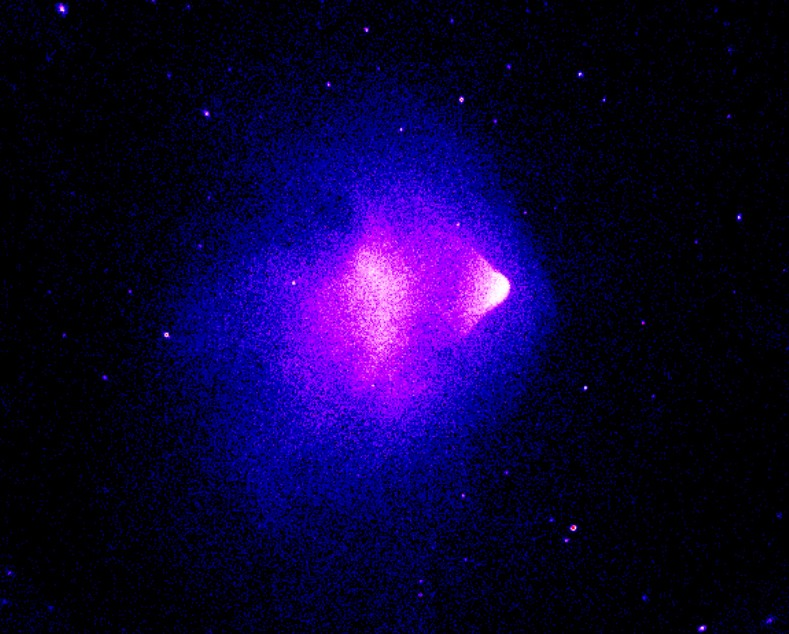
\includegraphics[scale=0.2]{bclstr.jpg}
\end{column}

\end{columns}
\end{frame}




%\begin{frame}{Types of Dark Matter}
%On the basis of the velocity of the Dark matter, it is devided into two types.
%
%\begin{itemize}
%\item \textbf{Cold Dark Matter:} Non-relativistic speed at the time of decoupling.
%
%\item \textbf{Hot Dark Matter:} Relativistic speed at the decoupling.
%\end{itemize}
%
%\end{frame}


\begin{frame}{Properties of Dark Matter known so far}

\section{Properties of Dark Matter known so far}

\begin{itemize}


\item From astrophysical and cosmological observations so far, the Dark Matter has gravitational interaction and no electromagnetic and strong interactions.
\vspace{2mm}
%\item Dark Matter can not have strong interaction as they are non-baryonic which comes from observations.

%\item It has gravitational interaction.

\item \textcolor{orange}{But the possibility of the dark matter having weak interaction has not been discarded by those observations.}
\vspace{2mm}
\item We still don't have any particle physics explanation of the Dark Matter.
\vspace{2mm}

\item To understand the nature of the Dark Matter has become an active field of research in high energy physics, astrophysics and cosmology.
%\item We are interested in cold dark matter.

\end{itemize}
\end{frame}


%\begin{frame}{Dark Matter searches}
%There are essentially three different ways to detect Dark Matter.
%\begin{enumerate}
%\item \textbf{Collider searches:} Two Standard Model Particles collide with each other and produce Dark Matter and this production resulted in missing energy.
%
%\item \textbf{Direct detection:} In this technique, one seaches for the recoils of different types of matter due to interaction with the Dark Matter.
%
%\item \textbf{Indirect detection:} In this case, we detect the produced particles in the process of dark matter self annihilation.
%\end{enumerate}
%
%\end{frame}




\begin{frame}[t]{Dark Matter searches}

\section{Dark Matter searches}
\begin{small}
\begin{columns}
\begin{column}{0.6\textwidth}
\begin{enumerate}

\item \textbf{Collider searches:} Two Standard Model Particles collide with each other and produce Dark Matter and this production resulted in missing energy.

\item \textbf{Direct detection:} In this technique, one seaches for the recoils of different types of matter due to interaction with the Dark Matter.

\item \textbf{Indirect detection:} In this case, we detect the produced particles in the process of dark matter self annihilation.

\end{enumerate}
\end{column}

\begin{column}{0.4\textwidth}
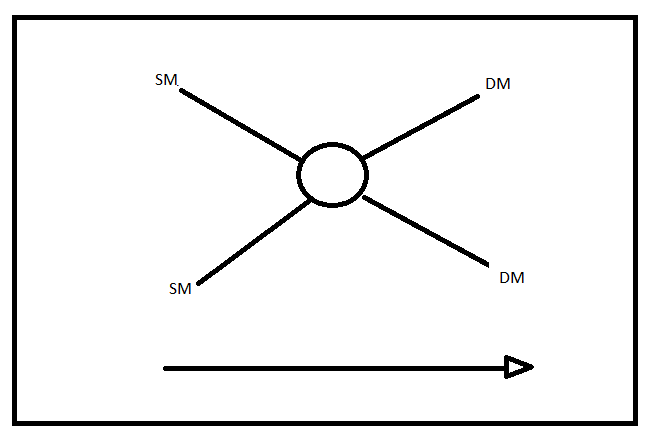
\includegraphics[scale=0.14]{collider_searches1.png}\\

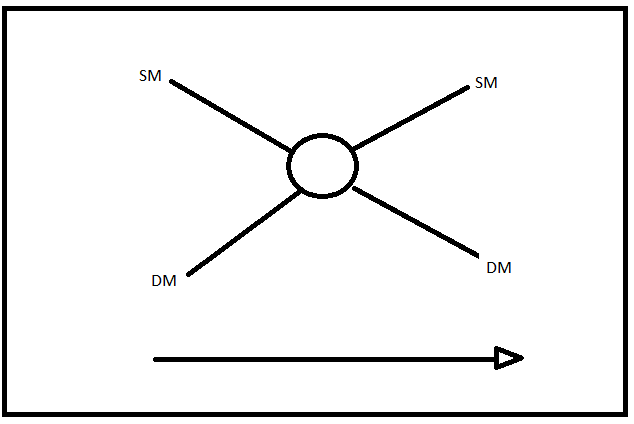
\includegraphics[scale=0.14]{Direct_detection1.png}\\

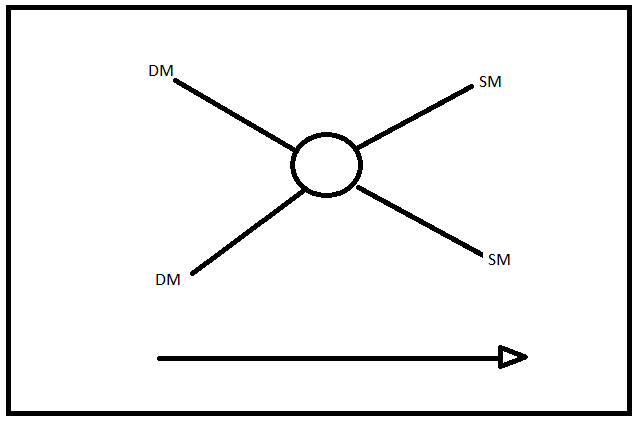
\includegraphics[scale=0.14]{indirect_detection1.png}\\

\end{column}



\end{columns}

\end{small}
\end{frame}








\begin{frame}{Dark Matter Indirect Detection}

\section{Dark Matter Indirect Detection}
\begin{itemize}


\item Dark Matter annihilating into energetic gamma rays at the center of the galaxy is its promising indirect detection signal.

\item The gamma ray flux relevant for the indirect detection is given by the following formula:

\begin{equation*}
\frac{d\phi}{dE} =  \frac{1}{4 \pi}\; \frac{<\sigma v> }{2 m^2_\chi} \left(\frac{dN}{dE}\right)_0 \int_{\Delta\Omega} \int_{LOS} dr\; d\Omega \rho^2(r) \label{indeq}
\end{equation*}


%\item Here $\left(\frac{dN}{dE}\right)_0$ denotes energy spectrum of each annihilation process, $<\sigma v> $ denotes thermally averaged cross-section times velocity, $m_\chi$ denotes the mass of the Dark Matter and $\rho(r)$ is the density profile of the Dark Matter, which we get from observation.\\
\item Here,
	\begin{itemize}
	\item $<\sigma v> $ is thermally averaged cross-			section times velocity.
	\item $m_\chi$ is the mass of the Dark Matter.
	\item $\left(\frac{dN}{dE}\right)_0$ is energy 			spectrum of each annihilation process.
	\item $\rho(r)$ is density profile of the dark 			matter.
	\end{itemize}

\item \textcolor{red}{ $<\sigma v>/ m^2_\chi$ depends on the Particle nature of the Dark Matter, which is the main focus of this thesis.}
%\textcolor{red}{This expression is simple as we are only considring the signals for neutral particles.}
	\end{itemize}

\end{frame}









\begin{frame}{Effective Field Theory Approach}

\section{Effective Field Theory Approach}

\begin{itemize}

\item \textcolor{teal}{We consider the simplest DM candidate, the Standard Model(SM) real scalar singlet and the interaction between DM and SM is treated in the framework of effective field theory (EFT)}.
\item \textcolor{red}{In the framework of the EFT, interaction terms in the lagrangian is written
as an expansion of its degrees of freedom and some couplings and a term $\Lambda$ which cut-off of our theory.}
\item \textcolor{blue}{Mass dimension of $\Lambda$ is $1$ and couplings are dimensionless.}
\item \textcolor{green}{EFT lagrangian can be written as:} $\mathscr{L}_{EFT}= \sum_{\mathscr{D}\geq 0} \frac{\mathscr{L}_\mathscr{D}}{\Lambda^{(\mathscr{D}-4)}}= \sum_{\mathscr{D}\geq 0 ,i} \frac{c_i^{(\mathscr{D})}\; \mathcal{O}_i^{(\mathscr{D})}}{\Lambda^{(\mathscr{D}-4)}}$


\end{itemize}
\end{frame}








\begin{frame}{EFT operators}

\section{EFT operators}

We construct EFT operators for the following processes:\\ 
DM DM$\longrightarrow q \bar{q}$, DM DM $\longrightarrow W^+W^-$, DM DM $\longrightarrow ZZ$, \\DM DM $\longrightarrow \gamma \gamma$, DM DM $\longrightarrow \gamma Z$.
\begin{center}
\begin{tabular}{|c|c|c|}
\hline
Label & Operators & Mass Dimension\\ \hline
$\mathcal{O}_1$ & $\frac{c}{\Lambda} \phi^2 \bar{q}q $ & $5$\\ \hline
$\mathcal{O}_2$ & $\frac{c_1}{\Lambda^2} \phi^2 W_{\mu \nu a} W^{\mu \nu}_a$ & $6$ \\ \hline

$\mathcal{O}_3$ & $\frac{c_2}{\Lambda^2} \phi^2 B_{\mu \nu} B^{\mu \nu}$ & $6$\\ \hline
\end{tabular}
\end{center}

* The cut-off $\Lambda$ has mass dimension $1$ and couplings are dimensionless.
\end{frame}


%\begin{frame}{Indirect Detection}
%To compute photon flux in indirect detection, we have the following formula:
%
%\begin{equation}
%\frac{d\phi}{dE} = \left(\frac{dN}{dE}\right)_0 \frac{1}{4 \pi}\; \frac{<\sigma v> }{2 m^2_\chi} \int_{\Delta\Omega} \int_{LOS} dr\; d\Omega \rho^2(r) \label{indeq}
%\end{equation}
%
%
%Here $\left(\frac{dN}{dE}\right)_0$ denotes energy spectrum of each annihilation process, $<\sigma v> $ denotes thermally averaged cross-section times velocity,
%$m_\chi$ denotes the mass of the Dark Matter and $\rho(r)$ is the density profile of the Dark Matter, which we get from observation.\\
%\textcolor{blue}{\textbf{We are interested in computing thermally averaged cross section times velocity which is almost equal to cross-section times velocity as the velocity is non-relativistic.}}
%\end{frame}
%




\begin{frame}{Interaction vertices}

\section{Interaction vertices}
To compute cross-sections from our EFT operators, we need the vertex factors for different operators. Recalling that we do not need to consider the mediator, we will consider point interaction.
In general to compute the vertex factors, we have the following formula for n-point interaction vertex in momentum space:

\begin{equation*}
V_{\phi_a(q_1) \phi_b(q_2)...\phi_c(q_n)} = \frac{\delta^nS_{eff}}{\delta \phi_a(q_1) \delta\phi_b(q_2)... \delta \phi_c(q_n)}
\end{equation*}

\end{frame}







\begin{frame}{Interaction vertices}
Applying this equation we get the following vertices from our EFT operators:
\vspace{0.5cm}

\begin{tiny}

\begin{tabular}{|c|c|c|}
\hline
Process & Notation & Vertex factor \\ \hline
\textbf{DM DM $\longrightarrow W^+W^-$ :}  & $ V_{\phi(k) \phi(k^\prime) W^{+\rho}(p) W^-_\sigma(p^\prime)} $ & $\frac{16c_1}{\Lambda^2} \{(p\cdot p^\prime) g_\rho^{\;\sigma}-p^{\prime \sigma} p_\rho\} \label{wv}$\\ \hline
\textbf{DM DM $\longrightarrow ZZ$:} & $
V_{\phi(k) \phi(k^\prime) Z^\sigma(p) Z_\rho(p^\prime)}  $ & $-\frac{8c^\prime}{\Lambda^2} \left\{ (p.p^\prime) g^\rho_{\sigma} - p_\sigma p^{\prime \rho} \right\} \label{zv}$  \\ \hline

\textbf{DM DM $\longrightarrow \gamma \gamma$:} & $ V_{\phi(k) \phi(k^\prime) \gamma_\rho(p) \gamma^\sigma(p^\prime)}$ & $ -\frac{8c_0}{\Lambda^2} \left\{ (p\cdot p^\prime) g^\rho_{\; \sigma }- p^{\prime \rho} p_\sigma \right\} \label{gv} $ \\ \hline

\textbf{DM DM $\longrightarrow \gamma Z$:} & $ V_{\phi(k) \phi(k^\prime) A_\rho(p) Z^\sigma(p^\prime)} $ & $ -\frac{8\tilde{c}}{\Lambda^2} \{ (p.p^\prime) g^\rho_{\; \sigma} - p^{\prime \rho} p_\sigma \} \label{gzv} $ \\ \hline
\end{tabular}

\end{tiny}

Here,
\begin{itemize}
\item $c^\prime = c_1\cos^2\theta_w+c_2\sin^2\theta_w$
\item $c_0 = c_1\sin^2\theta_w +c_2 \cos^2\theta_w$
\item $\tilde{c}= c_1 c_2 \cos\theta_w \sin\theta_w $
\end{itemize}


\end{frame}








\begin{frame}{Annihilation Cross-section}
\section{Annihilation Cross-section}
Now we computed the following cross-section at the non-relativistic approximation:


\begin{tiny}

\begin{tabular}{|c|}
\hline
 \textcolor{red}{\textbf{DM DM$\longrightarrow q \bar{q}$ :}} \\ \textcolor{blue}{$<\sigma v > \approx \frac{1}{16 \pi} \frac{c^2}{\Lambda^2} (1-\frac{m_q^2}{m_\chi^2})^{3/2} 
\left(1+ \frac{m_\chi^2 +2m_q^2}{m_\chi^2-m_q^2} \frac{v^2}{2}\right) \label{qqcross}$} \\ \hline

\textcolor{red}{\textbf{DM DM $\longrightarrow W^+W^-$:}}  \\ \textcolor{blue}{$<\sigma v> \approx \frac{4c^2_1}{3 \pi \Lambda^4}  \frac{1}{m^2_\chi}  \sqrt{1-\frac{m^2_w}{m^2_\chi}} \left[ m^4_w + 2(2 m^2_\chi -m^2_w)^2 + \right. $} \\ 
 \textcolor{blue}{$ \left. \left\{ \frac{ m^6_w+2 m^2_w (2 m^2_\chi - m^2_w)^2 }{2(m^2_\chi - m^2_w)} -\frac{m^4_w}{2} + (2 m^2_\chi - m^2_w) + 4 m^2_\chi (2 m^2_\chi - m^2_w)^2 \right\} v^2  \right]  \label{wwcross} 
$} \\ \hline
 

\textcolor{red}{\textbf{DM DM $\longrightarrow ZZ$:}}\\  \textcolor{blue}{$<\sigma v> \approx \frac{4c^\prime_1}{3 \pi \Lambda^4}  \frac{1}{m^2_\chi}  \sqrt{1-\frac{m^2_z}{m^2_\chi}} \left[ m^4_z + 2(2 m^2_\chi -m^2_z)^2 + \right.$} \\ 
\textcolor{blue}{$\left. \left\{ \frac{ m^6_z+2 m^2_z (2 m^2_\chi - m^2_z)^2 }{2(m^2_\chi - m^2_z)} -\frac{m^4_z}{2} + (2 m^2_\chi - m^2_z) + 4 m^2_\chi (2 m^2_\chi - m^2_z)^2 \right\} v^2  \right] \label{zzcross}$} \\ \hline


\textcolor{red}{\textbf{DM DM $\longrightarrow \gamma \gamma$:}}\\
\textcolor{blue}{$<\sigma v> = \frac{4}{\pi} \frac{c^2_0}{\Lambda^4} m^2_\chi \left(1+\frac{3}{2} v^2 \right) \label{ggcross}$} \\ \hline


\textcolor{red}{\textbf{DM DM $\longrightarrow \gamma Z$:}} \\
\textcolor{blue}{$<\sigma v> \approx \frac{1}{\pi} \frac{\tilde{c}^2}{\Lambda^4} m^2_\chi \left( 1- \frac{m^2_z}{4 m^2_\chi} \right)^3 \left\{1 + \frac{4m^2_\chi - 3m^2_z}{(4m^2_\chi - m^2_z)} v^2\right\} \label{gzcross}$} \\ \hline
\end{tabular}


\end{tiny}

\end{frame}






\begin{frame}{Results \& Discussion}
\section{Results \& Discussion}
\vspace{-4mm}

\begin{small}

\begin{itemize}

\item All the cross-sections are velocity unsuppressed.
\vspace{-1mm}
\item Our benchmark values are $c_1=c^\prime = \tilde{c}=0.5$ and the cutt-off to $100 \; TeV$ we plot the following s-wave result:


\begin{tabular}{cc}
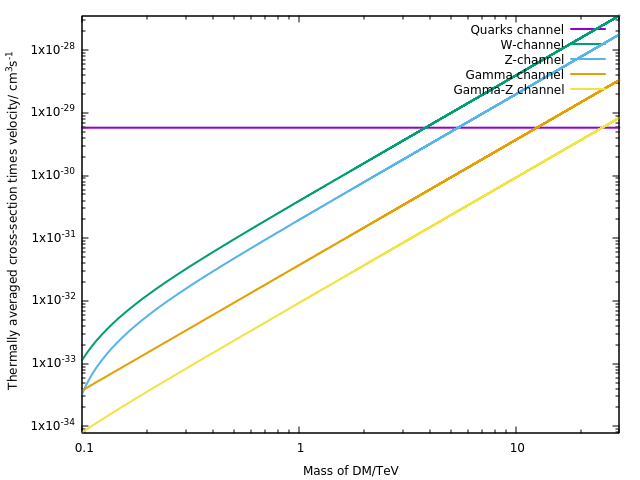
\includegraphics[scale=0.28]{CR1.png} & 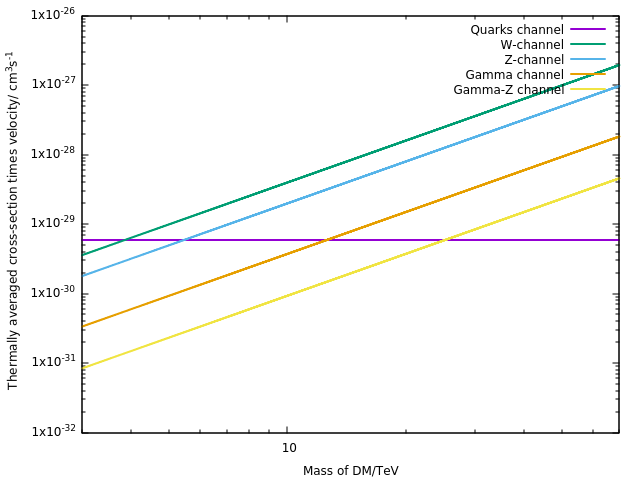
\includegraphics[scale=0.28]{CR2.png} \\

Mass $100\; GeV$ to $30\; TeV$ & Mass $3\; TeV$ to $70\; TeV$ 
\end{tabular}


\end{itemize}

\end{small}

\vspace{-4mm}
\begin{small}
\begin{itemize}
\item Here below DM mass range $m_\chi \sim 3.7 \;TeV$ quarks channel is relevant and above this the W-boson channel becomes dominant. 
\vspace{-1.5mm}
\item It should be noted here
that the intersection points in the graph actually depends on the couplings and the cutt-off we set in our
theory. 

\end{itemize}
\end{small}

\end{frame}

\end{document}